\documentclass[twocolumn]{article}
\usepackage{color
}
\usepackage{cite}
\usepackage{draftwatermark}
\usepackage{multirow}
\usepackage{listings}
\usepackage{float}
\usepackage{amsfonts}
\usepackage{amssymb}
\usepackage{amsmath}
\usepackage{amsthm}
\usepackage{epsfig}
\usepackage{epstopdf}
\usepackage{titling}
\usepackage{url}
\usepackage{enumitem}
\usepackage{array}
\usepackage[utf8]{inputenc}
\usepackage[english]{babel}
\usepackage{tikz}
\usepackage{algorithm}
\usepackage[noend]{algpseudocode}
\usepackage{abstract}
\usepackage[inkscapeformat=png]{svg}
\definecolor{pagecolor}{rgb}{1,1,1}
\pagecolor{pagecolor}

\usetikzlibrary{shapes,arrows,positioning,patterns,through}
\SetWatermarkText{Preview}
\SetWatermarkScale{1}
\setlength\parskip{.5\baselineskip}

\tikzset{
  dot node/.style={
    shape=circle,
    fill=white,
    draw,
    inner sep=+0pt,
    minimum size=+5mm
  },
  dotdot node/.style 2 args={
    dot node,
    label={[shape=circle,fill=black,outer sep=+0pt,inner sep=+0pt,minimum size=+3mm,name=ddd-#1,#2]center:}
  },
  arc style/.style={
    |<->|,
    shorten >=+-.5\pgflinewidth,
    shorten <=+-.5\pgflinewidth,
  }
}
\author{
  CTO of Rings Network \\ 0xea@ringsnetwork.io \\ \\
  \and
  Architect of Rings Network \\ 0xca@ringsnetwork.io
}

\title{BNS - A Sovereign DNS Based on Rings Network}

\begin{document}
\twocolumn[
  \begin{@twocolumnfalse}

\maketitle
    \begin{abstract}

This paper presents a DID method\cite{W3C-DID-Core} built with dDNS\cite{dns}(distributed DNS) and a new data transfer infrastructure based on Rings Network. Rings Network is a peer-to-peer network based on Chord algorithm it can be used to provide extendable DNS service and secure network traffic for traditional web2 and web3 applications on blockchains. The nodes of Rings Network can run on servers and in browsers(as WebAssembly\cite{webassembly}) and nodes in browsers and servers are functionally equivalent. This paper will describe how to implement DID proofs, DID Controller, and scalable DID Document based on Rings Network and demonstrate some possibilities of the application layer, such as utilizing the convenience of BNS for MPC and atomic swaps.


  ~\\
  ~\\
\end{abstract}

\end{@twocolumnfalse}
]

\section{Introduction and Motivation}
The increasing centralization of the internet is partly due to the loss of data sovereignty\cite{si} by individuals, which is reflected in the data monopolies of corporations and governments, as well as the fundamental architectural problem of the DNS system on the internet. The centralized structure of the current DNS system makes it susceptible to various security and privacy concerns, as well as scalability issues. Despite attempts to address these challenges with solutions like dDNS and DNSSEC, they have fallen short of providing a complete solution.


The issues stem from two primary considerations: first, the need to eliminate centralized resolution, where trust in decentralized proofs is preferred over reliance on central authorities when a subject asserts ownership of a domain; and second, the requirement to eliminate centralized services, where it is desired that the services hosted on the domain also become fully decentralized.

Therefore, we propose BNS, a decentralized domain name system based on Rings Network and blockchain technology. It consists of two parts, a chain-based resolution system based on smart contracts, and a DID interaction system based on Rings Network.

\subsection{Distributed DNS}

Accessing a host on the Internet typically involves two steps: domain name resolution and accessing the corresponding service. Traditionally, each of these steps is centralized. BNS aims to decentralize this process by offering decentralized domain name registration based on a distributed ledger and utilizing the Rings Network for domain name lookup and routing. The Rings Network is a peer-to-peer end-to-end network that is used to lookup the associated service for a domain name and ensure the privacy of traffic and decentralization of hosted services.

The figure \ref{dht} depicts the prototype of the Rings DHT, which enables the resolution of domains into various services, including direct messages with users, hosted websites, and provided services, among others.

\begin{figure*}[]
  \label{dht}
  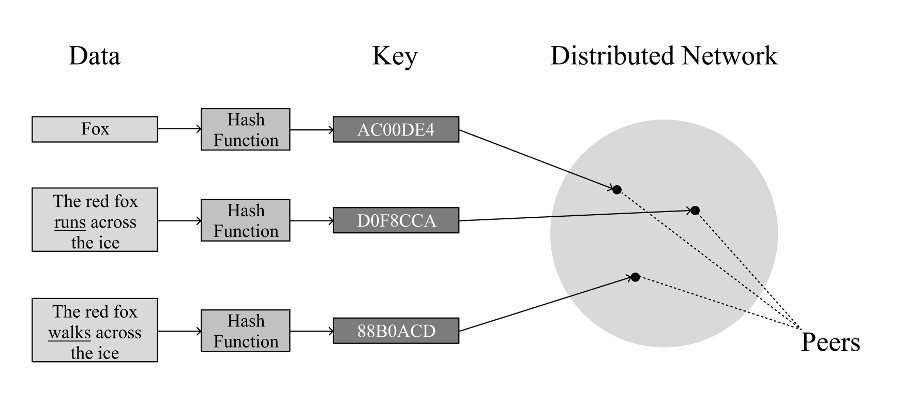
\includegraphics[width=\linewidth]{imgs/1.png}
  \caption{DHT Prototype.}
\end{figure*}



\subsection{DID Methods}

With the assistance of Rings Network, BNS has the potential to be the most powerful DID (Decentralized Identifier) method in history. According to the definition of DID in W3C's DID use case, a DID should meet the following four requirements:

\begin{itemize}[itemsep=2pt,topsep=0pt,parsep=0pt]
\item    decentralized: there should be no central issuing agency;
\item    persistent: the identifier should be inherently persistent, not requiring the continued operation of an underling organization;
\item    cryptographically verifiable: it should be possible to prove control of the identifier cryptographically;
\item    resolvable: it should be possible to discover metadata about the identifier.
\end{itemize}

Despite the large number of experimental DID method specifications (103) and implementations (32)\cite{W3C-DID-Use-Cases}, there are very few DIDs that have passed the DID test cases. Out of the 17 Ethereum-related DIDs (etho, ethr, ens, erc725, etc.), only ethr has met the standards set by the W3C for DIDs.

The BNS is a new DID (Decentralized Identifier) Method, with its DID schema specified as follows: did:bns:<protocol>:<did>.btc. The suffix "btc" represents the domain name extension of BNS, while the "protocol" component supports a variety of services, including HTTP, IM, and wallet.

\subsection{DID Proofs}
DID proofs refer to how the relationship between the did controller and the did document is proved. For some DIDs such as ENS (although they do not pass the standard, we discuss them as such because of the widespread interest), the did document refers to what the user writes into the distributed ledger, but for BNS it will include an additional part: the part in the Rings DHT where the did controller will be able to register and update the protocol and services provided by the DID through the Rings Network to register and update the protocols and services provided by the DID. So our DID proofs are more flexible and versatile than ENS, it supports any kind of cryptographic proofs, we have the implementation of secp256k1 and ed25519 curves now, and more in the future.

\begin{figure}[H]
  \label{arch}
  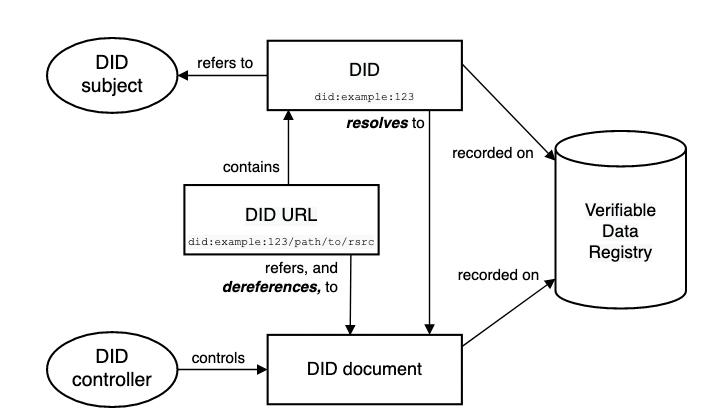
\includegraphics[width=\linewidth]{imgs/arch.png}
  \caption{OvervieDID archiecture}
\end{figure}

figure \ref{arch} shows the relationship between DID controller, DID document and DID subject.

\section{Related Work}


Chord can provide the same service by converting each hostname to a key. Chord-based\cite{chord} DNS does not require special servers, while normal DNS relies on a special set of root servers. DNS requires manual management of routing information (NS records) that allow clients to navigate a hierarchy of nameservers; Chord automatically maintains the accuracy of analog routing information. DNS works correctly only if the hostname structure reflects administrative boundaries; Chord does not enforce a naming structure. While DNS is specialized for the task of finding named hosts or services, Chord can also be used to find data objects that are not tied to a specific machine.

Pastry is an overlay network and routing network for the implementation of a distributed hash table (DHT) similar to Chord. The key-value pairs are stored in a redundant peer-to-peer network of connected Internet hosts. The protocol is bootstrapped by supplying it with the IP address of a peer already in the network and from then on via the routing table which is dynamically built and repaired. It is claimed that because of its redundant and decentralized nature there is no single point of failure and any single node can leave the network at any time without warning and with little or no chance of data loss. The protocol is also capable of using a routing metric supplied by an outside program, such as ping or traceroute, to determine the best routes to store in its routing table.

Freenet is a peer-to-peer platform for censorship-resistant, anonymous communication. It uses a decentralized distributed data store to keep and deliver information and has a suite of free software for publishing and communicating on the Web without fear of censorship. Both Freenet and some of its associated tools were originally designed by Ian Clarke, who defined Freenet's goal as providing freedom of speech on the Internet with strong anonymity protection.

The Globe system has a wide-area location service to map object identifiers to the locations of moving objects. Globe arranges the Internet as a hierarchy of geographical, topological, or administrative domains, effectively constructing a static worldwide search tree, much like DNS. Information about an object is stored in a particular leaf domain, and pointer caches provide search shortcuts. The Globe system handles a high load on the logical root by partitioning objects among multiple physical root servers using hash-like techniques. Chord performs this hash function well enough that it can achieve scalability without also involving any hierarchy, though Chord does not exploit network locality as well as Globe.

PNRP(Peer Name Resolution Protocol) is a peer-to-peer protocol designed by Microsoft. PNRP enables dynamic name publication and resolution and requires IPv6. PNRP was first mentioned during a presentation at a P2P conference in November 2001. Other hosts can then resolve the peer name, retrieve the corresponding addresses and other information, and establish peer-to-peer connections. Internally, PNRP uses an architecture similar to distributed hash table systems such as Chord or Pastry. The cache maintenance algorithm ensures that each node maintains adequate knowledge of the "cloud". It is designed to ensure that the time to resolve a request varies as the logarithm of the size of the cloud. PNRP now works on the released Windows systems but no evidence shows it could be used on other platforms.

DoX is a peer-to-peer DNS networking method for detecting and correcting inaccurate DNS records caused by cache poisoning attacks. DoX uses Chord to store and synchronize hostnames and keys. Only detecting or correcting is the solution after the problem occurs. We believe that using crypto algorithms to verify and transfer data among nodes is better and safer. Two-way hostname data synchronization between DNS network and blockchain datastores is necessary for long-term data storing and full decentralized implementation.

Onion Routing(the core principle of Tor\cite{TorNetwork}) is implemented by encryption in the application layer of the communication protocol stack. As Tor cannot encrypt the traffic between an exit node and the target server, any exit node is in a position to capture traffic passing through it that does not use end-to-end encryption such as Secure Sockets Layer (SSL) or Transport Layer Security (TLS). Shreds of evidence show that hackers can exploit usernames and passwords for email accounts by operating and monitoring Tor exit nodes.
\section{System Design}

We will describe how the system works in two parts, firstly the operation of DNS and secondly the function of DID in the DHT network.
\subsection{dDNS implementation}
Our system handles lookups at the granularity of resource record sets (RRSets), as in conventional DNS. An RRSet is a list of all the records matching a given domain name and resource type.
DNSSEC uses public-key cryptography to sign re-source record sets. When we retrieve an RRSet from an arbitrary server, we need to verify the signature (included as a signature (SIG) record). To find the public key that should have signed the RRSet, we need to execute another DNS lookup, this time for a public key (KEY) RRSet. This RRSet is in turn, signed with the public key for the enclosing domain.
\begin{figure*}[H]
  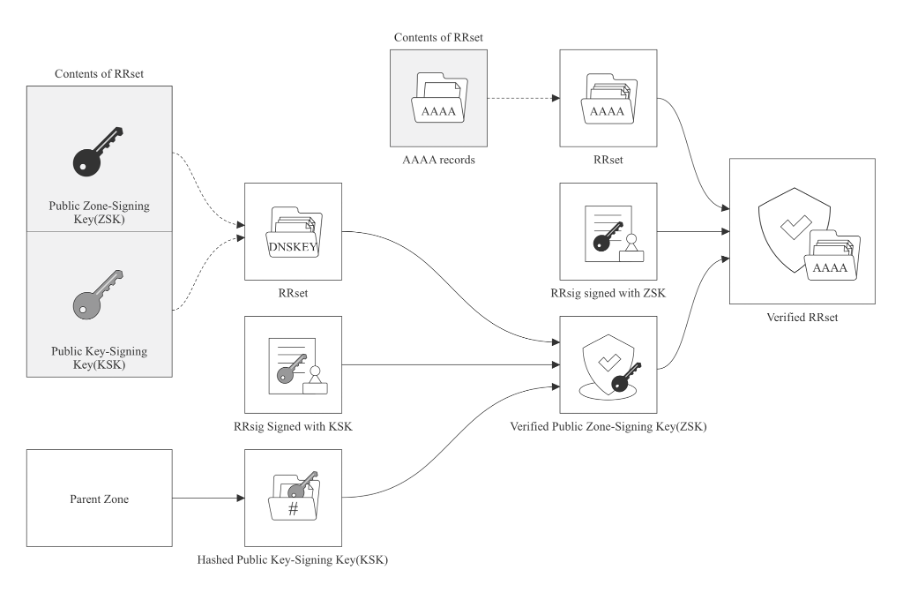
\includegraphics[width=\linewidth]{imgs/2.png}
    \caption{DNS}
\end{figure*}
\begin{figure}[htbp]
  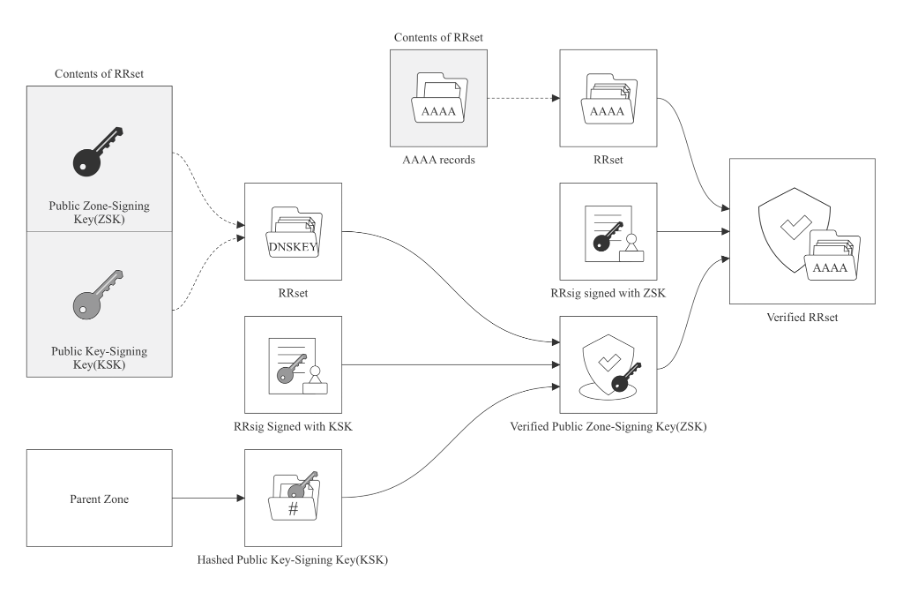
\includegraphics[width=\linewidth]{imgs/4.png}
  \caption{dDNS}
  \label{ddns}

  \end{figure}


dDNS stores and retrieves resource record sets using DHash, a Chord-based distributed hash table. DHash has two properties useful for this discussion: load balance and robustness.

DHash uses consistent hashing to allocate keys to nodes evenly. Further, as each block is retrieved, it is cached along the lookup path. If a particular record is looked up n times in succession starting at random locations in a Chord ring of m nodes, then with high probability, each server transfers a given record only log m times total before every server has the record cached.
DHash is also robust: as servers come and go, DHash automatically moves data so that it is always stored on a fixed number of replicas (typically six). Because the replicas that store a block are chosen in a pseudo-random fashion, a very large number of servers must fail simultaneously before data loss occurs.

To create or update a DDNS RRSet, the owner prepares the RRSet, signs it, and inserts it into DHash. The key for the RRSet is the SHA1 hash of the domain name and the RRSet query type.

Naively verifying a DNS RRSet for a name with n path elements requires n KEY lookups. We address this problem by allowing the owner to present additional relevant KEYs in the RRSet. To avoid inflating the responses, we can omit KEY RRSets for popular names.

To ease the transition from conventional DNS to our system, a simple loopback server listening on 127.1 could accept conventional DNS queries, perform the appropriate Chord lookup, and then send a conventional response. Then systems could simply be configured to point at 127.1 as their name server.

\subsection{BNS lookup protocol}

BNSLS (BNS lookup service) is based on Rings Network, which queries, searches, and resolves services through Rings DHT. Since Rings Network's network layer is based on WebRTC\cite{webrtc-standard} and WASM, BNS provides a browser-based, DID-to-DID access channel. Figure \ref{RTC} shows how the node is connected directly via RTCPeerConnection. An RTCPeerConnectioninstance allows an application to establish peer-to-peer communications with another RTCPeerConnection instance in another browser, or to another endpoint implementing the required protocols. Communications are coordinated by the exchange of control messages (called a signaling protocol) over a signaling channel which is provided by unspecified means.

Based on the Rings DHT, the BNS allows the DIDs to better lookup each other, which may include the person behind the DID, the machine behind the DID, the service, or a subnet consisting of a Rings network - which will usually also have a DID.
\begin{figure}[htbp]
  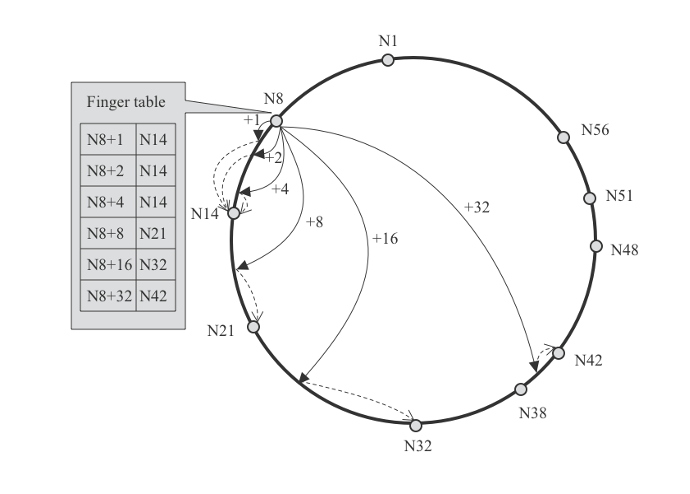
\includegraphics[width=\linewidth]{imgs/chord.png}
  \caption{Rings DHT}
  \label{chord}

  \end{figure}

Rings DHT is a variant of Chord DHT that stores the BNS domain on a ring structure and allows the BNS controller to register and discover other services. The \ref{chord} figure shows how a rings node stores nearby DIDs.


\subsection{DNS Provider}
BNS supports a wider range of applications and scenarios by providing web extensions and JSON-RPC. As the Rings Network is a browser-native network, it enables many applications based on WebAssembly (WASM) to run directly in the user's browser.

BNS Providers run a full node of the Rings Network on the backend and inject themselves into window.rings.bns, allowing users to directly access BNS's DNS resolver through the Rings Provider, thereby enabling access to the desired decentralized applications.
\subsection{DID Protocol}

As a DID Method, BNS provides a scalable and secure method for managing DID Documents by leveraging both distributed ledger technology and a decentralized network. This allows for a more reliable and secure solution compared to traditional centralized approaches. The BNS DID syntax conforms to the specifications defined by the World Wide Web Consortium (w3c) and extends to support various protocols and DID URLs. The integration of Rings Network into BNS further enhances its capabilities by abstracting the DID into a mathematically finite ring. This enables BNS to easily perform complex cryptographic operations, such as constructing secret sharing schemes based on Shamir's Secret Sharing (SSSS) technique. Additionally, this abstraction also allows for greater privacy and security as well as a more decentralized approach to DID document management.


\begin{figure}[htbp]
  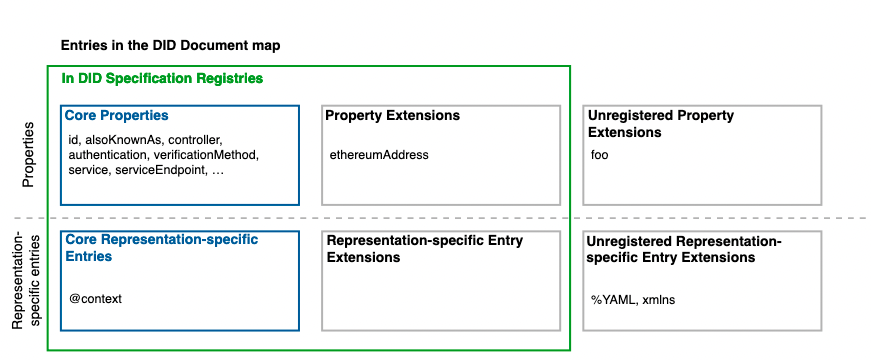
\includegraphics[width=\linewidth]{imgs/diddoc.png}
  \caption{Did Document}
  \label{diddoc}

\end{figure}

figure \ref{diddoc} shows the basic structure of a DID Document.

BNS offers a flexible extension to DID Documents, using the BNS DID Controller, users can implement decentralized web and service registration, service discovery, and other functions through the Rings Network. Additionally, interactions such as atomic swaps and multi-signatures can be achieved through DID discovery between DID Documents.


\section{Applications}

BNS as a DID Method offers very big possibilities for dweb and web3. We have also implemented several simple demos for it, including BNSChat, BNSWeb and atomic swap.


\textbf{BNSChat} is a secure and decentralized chat application that employs end-to-end encryption to facilitate direct browser-to-browser communication. Utilizing a Decentralized Identifier (DID) as a decentralized identity solution, users can easily establish peer-to-peer encrypted communication channels without the need for intermediaries. In scenarios where access to third-party nodes is not feasible, communication can still occur through the direct exchange of Session Description Protocols (SDPs).

\begin{figure}[htbp]
  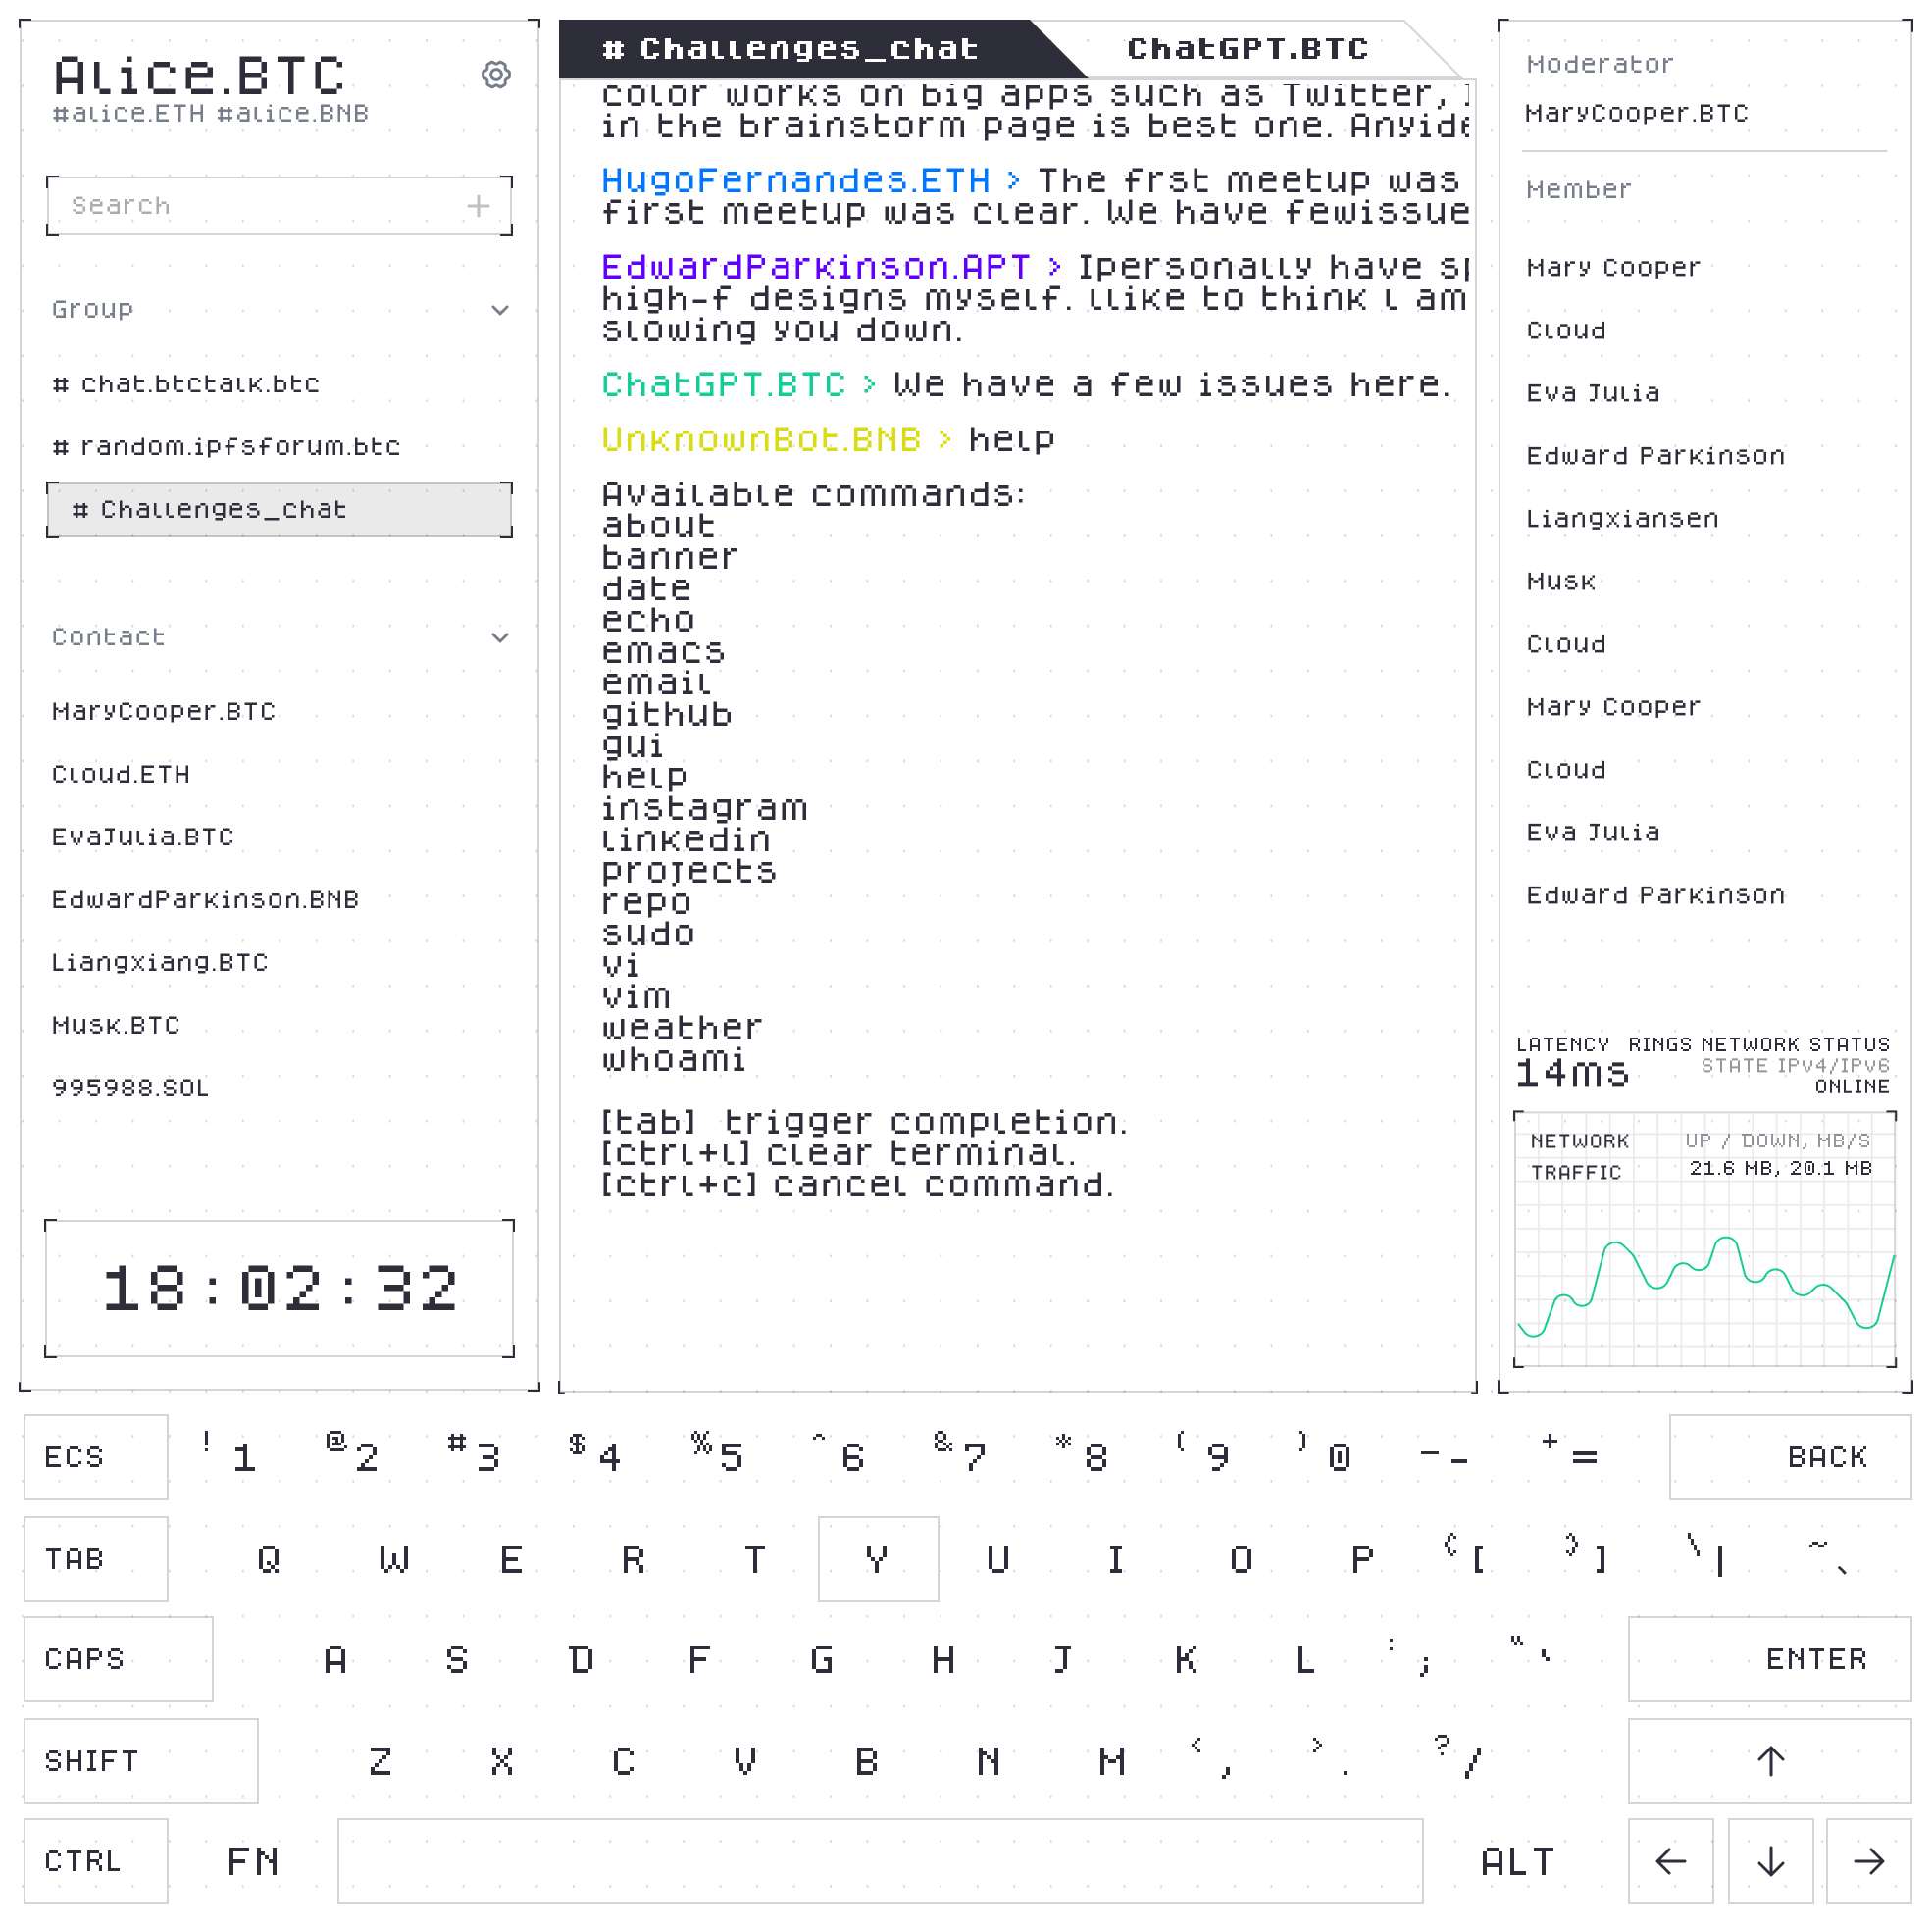
\includegraphics[width=\linewidth]{imgs/chat.jpg}
  \caption{BNSChat}
  \label{diddoc}

\end{figure}
Moreover, BNSChat utilizes the Rings Network to facilitate highly efficient interactions with other BNS holders, incorporating all the functionalities of an instant messaging platform and supporting atomic swaps, which will be further discussed.

\textbf{BNS Mailbox}: BNS implements anonymous email functionality through the Rings Network. When a user needs to send an email to a DID, they simply send the email to the anonymous mapping of that DID in the Rings DHT network. This process does not reveal any real information. The message is delivered to the corresponding Mailbox via a Relay, and the recipient retrieves the message by proving ownership and decrypting it from the Mailbox.

Retrieving messages through a DID is a safer method than direct messaging. BNS Mailbox helps DIDs establish highly anonymous and secure new channels for messages.

\textbf{BNS Web} is a decentralized web implementation modeled after the Tor network that enables users to access web information anonymously and bypass censorship. While BNS Web represents a small component of the BNS Service Register/Lookup Protocol, the protocol also offers Oracle API services based on BNS and the Rings Network, including APIs similar to those offered by Ethereum\cite{Ethereum}.

Web service providers, akin to the role of hidden services in the Onion Network, can use the Rings Network's service registration feature to register their DID-associated services to the DHT network, ensuring their services remain online permanently. This register/lookup process simply involves the DID controller modifying the DID document.

For instance, in BNS Web, a node might provide IPFS\cite{IPFS} services, and other nodes can discover these services through service discovery and directly access IPFS data through their browser. This is more convenient compared to traditional IPFS access methods that necessitate running an IPFS node on a local computer or relying on a centralized server.

The Rings Network's chunking and obfuscation of traffic effectively thwarts censorship and surveillance from centralized organizations on DIDs, significantly boosting privacy.

\textbf{BNS Secret Sharing}

Based on the Rings Network, BNS can implement Secret Sharing using ElGamal\cite{ElGamalEncryption} and Rings DID. This is commonly referred to as the SSSS algorithm. An example is where a secret is divided into 3n parts, and it can only be revealed when more than 2n + 1 participants are willing to participate in the interaction.

The requirement for participants to engage in multiple rounds of interaction increases the difficulty of implementing secret sharing based on the SSSS algorithm. The lack of decentralized channels further adds to the feasibility of the SSSS algorithm on BNS and the Rings network.


\textbf{BNS Atomic Swap} Atomic swap is a pioneering cross-chain algorithm that has faced challenges in widespread adoption due to the need for frequent interactions and the absence of decentralized channels. For instance, classical atomic swaps require price negotiation, the exchange of swap IDs, and other similar steps. BNS effectively addresses these challenges through its robust decentralized peer-to-peer network.

Classical atomic swaps can be broken down into the following steps, as described in \cite{eth-atomic-swap}:

\begin{figure}
\[
\begin{array}{l l l}
  \text{\textbf{Alice}} & & \text{\textbf{Bob}} \\
    &\xleftarrow{Hash(sk)} & sk  \\
  open(id) & & \\
                        & \xleftarrow{confirm} & check(id) \\
                        & \xleftarrow{sk} & close(id) \\
  check(sk) & & \\
\end{array}
\]
\label{swap}
\caption{swap}
\end{figure}


\begin{itemize}[itemsep=2pt,topsep=0pt,parsep=0pt]

 \item   Both Alice and Bob agree on the terms of the swap, including the cryptocurrencies to be exchanged and the exchange rate.
\item    Alice generates a hash of the secret key and sends the hash to the other party, along with the terms of the swap.
\item     Bob confirms that it agrees to the terms of the swap, and sends its own hash of the secret key to the first party.
\item    Both Alice and Bob use the hashes to create a smart contract on their respective blockchains, locking in the swap.
\item    When both Alice and Bob have confirmed that the other party's funds have been locked in the smart contract, they can reveal the secret key.
\item    The atomic swap executed, automatically exchanging the funds.
\end{itemize}
We briefly describe the close, expire algorithm in atomic swaps.

\begin{algorithm}[htbp]
\caption{Close the Atomic Swap}
\begin{algorithmic}[1]
\Function{close}{$swapID$, $secretKey$}
\State \textbf{Input:} $swapID$ - the identifier of the atomic swap, $secretKey$ - the secret key associated with the swap
\State \textbf{Requirement:} The swap with identifier $swapID$ must be in 'Open' state and the caller must have the secret key associated with the swap
\State \textbf{Output:} Closes the atomic swap and transfers the funds
\State $swap \gets swaps[swapID]$
\State $swaps[swapID].secretKey \gets secretKey$
\State $swapStates[swapID] \gets \text{States.CLOSED}$
\State $swap.withdrawTrader.transfer(swap.value)$
\State \textbf{Trigger:} Close event with parameters ($swapID$, $secretKey$)
\EndFunction
\end{algorithmic}
\end{algorithm}

\begin{algorithm}[htbp]
\caption{Expire}
\begin{algorithmic}[1]
\Function{Expire}{$swapID$}
\State $swap \gets swaps[{swapID}]$
\State $swapStates[{swapID}] \gets States.EXPIRED$
\State $swap.ethTrader.transfer(swap.value)$
\State $\textbf{emit}$ Expire(${swapID}$)
\EndFunction
\end{algorithmic}
\end{algorithm}

\begin{algorithm}[htbp]
\caption{check(bytes32 $\text{swapID}$)}
\begin{algorithmic}[1]
\Function{check}{$\text{swapID}$}
\State $\text{swap} \gets \text{swaps[}\text{swapID}\text{]}$
\State \Return ($\text{swap.timelock, swap.value}$)
\State \Return ($\text{swap.withdrawTrader, swap.secretLock}$)
\EndFunction
\end{algorithmic}
\end{algorithm}

\begin{algorithm}[htbp]
\caption{checkSecretKey()}
\begin{algorithmic}[1]
\Function{checkSecretKey}{bytes32 ${swapID}$}
\State \textbf{public view onlyClosedSwaps}$({swapID})$
\State \textbf{returns (bytes memory secretKey)}
\State Swap memory swap = swaps[${swapID}$]
\State \textbf{return} swap.secretKey
\EndFunction
\end{algorithmic}
\end{algorithm}

\section{Conclusion}
Rings network aims to build a new generation of Internet infrastructure, integrating web2.0 and web3.0 (especially blockchain technology) to provide a new generation of decentralized Internet solutions. Humanity created the first generation of the Internet out of the need for easy information sharing. The broader need gave rise to infrastructures such as large server rooms, submarine fiber optic cables, and satellite communications. The human nature of creation and communication allowed web 2.0 to develop, but the basic functionality no longer met the demand. People need new financial systems and privacy systems. We desire independence, privacy, and ownership, we want knowledge to be preserved and passed on, and blockchain technology gives us hope.

Web3.0 shows us a new chapter of the Internet, where people expect a fairer, more democratic, and more accessible Internet in the face of political, geopolitical, nationalistic, and economic sanctions that block communication. rings network hopes to build a new generation of decentralized peer-to-peer networks based on cryptographic systems to make all this possible. We are just moving a small step forward on the shoulders of giants.

We do not oppose web2, blindly oppose centralization, nor do we oppose government regulation to protect the interests of the people. We respect all anarchists and those who oppose anarchism. However, we insist that technology is innocent. Those who create advanced technology are innocent. Only those who abuse technology to infringe on the rights and interests of others are guilty. Technology itself should not bear any crime.

The original intentions of the blockchain and the new generation of decentralized networks starting from Bitcoin\cite{Bitcin} are all good intentions, but we firmly believe that the principle of "Don't trust, verify it." can give us maximum security. We can’t trust anyone (including regulators, of course) to be kind, and to do the most optimistic things with the most pessimistic and malicious speculations will give us a brighter future.

The technology that can protect the privacy of the bad guys can protect the privacy of the good guys. Technology that can easily invade the privacy of bad guys can easily invade anyone's privacy. Cyber privacy is already a basic human right now, and we agree to bring the bad guys to justice, but not at the expense of everyone's rights.

We hope to provide web3 users with a sense of cybersecurity.


\bibliographystyle{unsrt}
\bibliography{./cites}
\end{document}